\documentclass[10pt, aspectratio=169]{beamer}
\usepackage{caption}
\usepackage{subcaption}
\usetheme[progressbar=frametitle]{metropolis}
\usepackage{amsmath}
\usepackage{siunitx}
\usepackage{xcolor}
\usecolortheme{crane}
\definecolor{craneorange}{rgb}{0.53,0.66,0.42}
\usecolortheme{spruce}
\usepackage{hyperref}
\usepackage{multimedia}
\usepackage[percent]{overpic}
\usepackage[para]{footmisc}

\title{Computational study of far-field acoustic emission by collapsing bubbles}
\date{\today}
\author[shortname]{Magu Raam Prasaad R}
\institute[shortinst]{Indian Institute of Science, Bangalore}

\begin{document}
\begin{frame}
	\maketitle
\end{frame}

\begin{frame}{Computational approach}
	
	\begin{itemize}
		\item In this work we compute the far-field acoustic waves emitted from bubble collapse process using the Kirchhoff integral formulation.
	\end{itemize}

	\begin{figure}
		\centering
		\includegraphics[scale=0.22]{images/shematic1.png}
		\caption{Schematic of far-field acoustic data computed from CFD solver using the Kirchhoff integral method.}
	\end{figure}		

\end{frame}

\begin{frame}{Kirchhoff integral formulation}
	\begin{columns}
		\column{0.5\textwidth}
		\begin{itemize}
			\item We chose a control surface $S$ that encloses all the acoustic sources, and the pressure perturbations $p'$ satisfies the homogeneous wave equation.
			\begin{equation}\label{Wave equation}
				\Bigg( \frac{1}{c_{0}^2}\frac{\partial{}^{2}}{\partial{t}^{2}}- \nabla{}^{2} \Bigg) p' = 0 \quad \quad \textrm{in} \ V.
			\end{equation}
			\item The control surface S is defined by $f(\mathbf{x}) = 0$, $f(\mathbf{x}) > 0$ for $\mathbf{x}$ in V and $f(\mathbf{x}) < 0$ for $\mathbf{x}$ inside surface S.
		\end{itemize}
				
		\column{0.5\textwidth}
		\begin{figure}[h]
			\includegraphics[scale = 0.3]{images/kirchhoff_surface.png}
			\caption{Stationary Kirchhoff surface $S$ encloses sound source}	
		\end{figure}
							
	\end{columns}
\end{frame}

\begin{frame}{Kirchhoff integral formulation}
	\begin{columns}
		\column{0.5\textwidth}
		\begin{itemize}
			\item We define the pressure $p'$ as a generalized function $pH(f)$ where
			\begin{equation*}\label{Generalized_Functions}
				p' H(f) =\begin{cases}
					p' , & \text{for $\mathbf{x}$ in V}.     \\
					0,  & \text{for $\mathbf{x}$ inside S}.
				\end{cases}
			\end{equation*}
			\item The acoustic wave equation in generalised pressure
			\begin{equation*}\label{Generalized Wave Equation}
				\Bigg( \frac{1}{c_{0}^2}\frac{\partial{}^{2}}{\partial{t}^{2}}- \nabla{}^{2} \Bigg) p'H = -\frac{\partial p'}{\partial n}\delta(f) - \nabla.(p' \mathbf{n} \delta(f)).
			\end{equation*}
		\end{itemize}
				
		\column{0.5\textwidth}
		\begin{figure}[h]
			\includegraphics[scale = 0.3]{images/kirchhoff_surface.png}
			\caption{Stationary Kirchhoff surface $S$ encloses sound source}	
		\end{figure}
							
	\end{columns}
\end{frame}

\begin{frame}{Kirchhoff integral formulation}
	\begin{itemize}
		\item The acoustic wave equation in generalized variables is valid in the
		entire unbounded space. Therefore we can use the free-space Green’s function to
		solve the equation.
		\begin{equation}\label{pressure}
			p'(\mathbf{x}, t) = \int s(\mathbf{y}, \tau){G(\mathbf{x}, t; \mathbf{y}, \tau )} d\mathbf{y}d\tau.
		\end{equation}
		where,
		\begin{equation}\label{Green's Function}
			G(\mathbf{x}, t; \mathbf{y}, \tau ) = \frac{\delta \Big(t - \tau - \frac{|\mathbf{x} - \mathbf{y}|}{c_{0}}\Big)}{4\pi|\mathbf{x} - \mathbf{y}|}
		\end{equation}
		and 
		\begin{equation}
			s(\mathbf{y}, \tau) = -\frac{\partial p'}{\partial n}\delta(f) - \nabla.(p' \mathbf{n} \delta(f)).
		\end{equation}
	\end{itemize}
\end{frame}

\begin{frame}{Kirchhoff integral formulation}
	\begin{itemize}
		\item Simplifying the equation further, we obtain the Kirchhoff integral equation for a stationary control surface
		\begin{equation}
			\begin{split}
				p'(\mathbf{x}, t) = -\frac{1}{4\pi}\int_{S}\Big[  \frac{p'}{r^{2}}\frac{\partial r}{\partial n} - \frac{1}{r}\frac{\partial p'}{\partial n} + \frac{1}{c r}\frac{\partial r}{\partial n}\frac{\partial p'}{\partial \tau} \Big]_{\tau} dS.
			\end{split} 
		\end{equation}
		$p'$ is the acoustic pressure satisfying the wave equation outside the control surface \textbf{S}, $c$ is the speed of sound at ambient conditions and $n$ is the normal.
		The integrands are evaluated at the emission time $\tau = t - \mathbf{r}/c$ and $\mathbf{r}= |\mathbf{x} - \mathbf{y}|$ is the distance between observer and source.
		\item The $p'$, ${\partial p'}/{\partial t}$ and ${\partial p'}/{\partial n}$ are computed from flow solver.
	\end{itemize}
\end{frame}

\begin{frame}{Kirchhoff integral on a cylinder}
	\begin{figure}
		\centering
		\includegraphics[scale=0.24]{images/cylinder.png}
		\caption{Cylindrical Kirchhoff surface}
	\end{figure}
\end{frame}

\begin{frame}{Kirchhoff integral on a cylinder}
	\begin{itemize}
		\item We compute the Kirchhoff integral on a cylindrical surface 
		\begin{equation}
			\begin{split}
				p'(r', z', t) =  -\frac{1}{4\pi}\int_{S_{top, bottom}}\Big[  \frac{p'}{r^{2}}&\frac{\partial r}{\partial n} - \frac{1}{r}\frac{\partial p'}{\partial n} + \frac{1}{c r}\frac{\partial r}{\partial n}\frac{\partial p'}{\partial \tau} \Big]_{\tau} r'dr'd\theta' \\
								 -\frac{1}{4\pi}\int_{S_{curved}} \Big[  \frac{p'}{r^{2}}&\frac{\partial r}{\partial n} - \frac{1}{r}\frac{\partial p'}{\partial n} + \frac{1}{c r}\frac{\partial r}{\partial n}\frac{\partial p'}{\partial \tau} \Big]_{\tau} Rd\theta'dz'  
			\end{split} 
		\end{equation}
		\item The above integral is numerically computed using Gauss quadrature
		\begin{equation}
			\begin{split}
				p'(r', z', t) =  -\frac{1}{4\pi}\sum_{i}^{N_r}\sum_{j}^{N_\theta}\sum_q^{Nqpts} \Big[  \frac{p'}{r^{2}}&\frac{\partial r}{\partial n} - \frac{1}{r}\frac{\partial p'}{\partial n} + \frac{1}{c r}\frac{\partial r}{\partial n}\frac{\partial p'}{\partial \tau} \Big]_{\tau} r'\Big |_q J_q w_q\\
								 -\frac{1}{4\pi}\sum_{j}^{N_\theta}\sum_{k}^{N_z}\sum_q^{Nqpts} \Big[  \frac{p'}{r^{2}}&\frac{\partial r}{\partial n} - \frac{1}{r}\frac{\partial p'}{\partial n} + \frac{1}{c r}\frac{\partial r}{\partial n}\frac{\partial p'}{\partial \tau} \Big]_{\tau} R \Big |_q J_q w_q 
			\end{split} 
		\end{equation}
		\item We use two-point Gauss quadrature on a reference cell $[-1, 1]\times [-1, 1]$. The quadrature points are mapped to computational cell using bi-linear interpolation. 
	\end{itemize}
\end{frame}

\begin{frame}{Kirchhoff integral on a cylinder}

	\begin{figure}
		\centering
		\includegraphics[scale=0.5]{images/quadpoints.png}
		\caption{Schematic of quadrature points on cylindrical surface}
	\end{figure}
\end{frame}


\begin{frame}{Results - Acoustic monopole}
	\begin{itemize}
		\item We solve the acoustic wave equation
		\begin{equation}
			\Bigg( \frac{1}{c_{0}^2}\frac{\partial{}^{2}}{\partial{t}^{2}}- \nabla{}^{2} \Bigg) p'(\mathbf{x}, t)  = -q(t)\delta(\mathbf{x}), 
		\end{equation}
		for a monopole source using the \textbf{Kirchhoff} method.
		\item And compare it with the exact solution $p'(\mathbf{x}, t) = -\frac{1}{4\pi} \frac{  q(t - \frac{r}{c_{0}}) }{r}$.
		\item We chose a monopole source
		\begin{equation}
			q(t) = 2(t - t0)f_{0}^{2}\exp( -f_{0}^2(t - t_{0})^{2}), 
		\end{equation}
		where $f_{0} = 100$ is the dominant frequency and $t_{0} = \frac{4}{f_{0}}$.
	\end{itemize}
\end{frame}

\begin{frame}{Results - Acoustic monopole}
	\begin{figure}
		\centering
		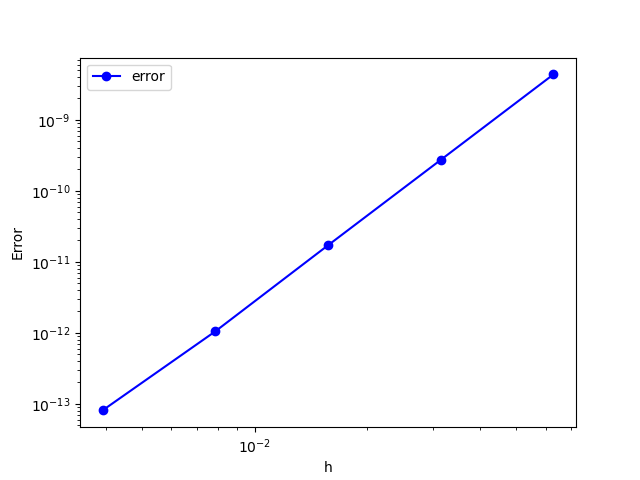
\includegraphics[scale=0.5]{images/convergence.png}
		\caption{We have obtained fourth-order convergence for the Kirchhoff integral computed using the two-point Gauss quadrature}
	\end{figure}
\end{frame}

\begin{frame}{Conclusion}
	\begin{itemize}
		\item In this work we have computed the acoustic waves emitted by a monopole source using the Kirchhoff method. And showed fourth-order convergence for the Kirchhoff integral computed using two-point Gauss quadrature.
	\end{itemize}
\end{frame}

\begin{frame}[standout]
	Thank you!
\end{frame}
\end{document}